%-------------------------------------------------------------------------------------------------------------------
\documentclass{beamer}
\usepackage{hyperref}
\usepackage[T1]{fontenc}
\usepackage{latexsym,amsmath,xcolor,multicol,booktabs,calligra}
\usepackage{graphicx,pstricks,listings,stackengine}
\usepackage{lipsum}
\usepackage{ragged2e}
\usepackage{blindtext}

%-------------------------------------------------------------------------------------------------------------------


%-------------------------------------------------------------------------------------------------------------------
\author{Instrutor: Mário Diego Rocha Valente \\
 \ \ \ \  \textbf{(Analista de Trânsito)}}
\title{Formação de Agentes de Fiscalização de Trânsito}
\subtitle{Disciplina: Mudanças no CTB}
\institute{
    Departamento de Trânsito do Estado do Pará \\
    Coordenadoria de Gestão e Recursos Humansos \\
    Gerência de Treinamento}
\date{Belém, 2022}
\usepackage{Ritsumeikan}

\def\cmd#1{\texttt{\color{red}\footnotesize $\backslash$#1}}
\def\env#1{\texttt{\color{blue}\footnotesize #1}}
\definecolor{deepblue}{rgb}{0,0,0.5}
\definecolor{deepred}{rgb}{0.6,0,0}
\definecolor{deepgreen}{rgb}{0,0.5,0}
\definecolor{halfgray}{gray}{0.55}

\lstset{
    basicstyle=\ttfamily\small,
    keywordstyle=\bfseries\color{deepblue},
    emphstyle=\ttfamily\color{deepred},    % Custom highlighting style
    stringstyle=\color{deepgreen},
    numbers=left,
    numberstyle=\small\color{halfgray},
    rulesepcolor=\color{red!20!green!20!blue!20},
    frame=shadowbox,}
%-------------------------------------------------------------------------------------------------------------------


%-------------------------------------------------------------------------------------------------------------------
\begin{document}
\begin{frame}
    \titlepage
    \begin{figure}[htpb]
        \begin{center}
            
\includegraphics[keepaspectratio, scale=0.017]{pic/Ritsumeikan_University_Logo.png}
        \end{center}
    \end{figure}
\end{frame}
\begin{frame}
    \tableofcontents[sectionstyle=show,subsectionstyle=show/shaded/hide,subsubsectionstyle=show/shaded/hide]
\end{frame}
%----------------------------------------------------------------------------------------------------------------------


%----------------------------------------------------------------------------------------------------------------------
\section{Lei n 14.071/2020}
\subsection{39 Mudança no CTB}
\begin{frame}{Fundamentos}
    \begin{itemize}
        \item \justifying Você conhece a Lei n 14.071/2020 – mais conhecida como Nova Lei de Trânsito?;
        \item \justifying Trata-se de uma lei proposta pelo Presidente Jair Bolsonaro, em 2019, que visava a fazer grandes mudanças no Código de Trânsito Brasileiro (CTB);
        \item \justifying Apresentado pelo Poder Executivo em junho de 2019, a Nova Lei iniciou seu caminho como Projeto de Lei n 3.267/2019, sobre o qual você provavelmente ouviu falar em algum momento;
        \item \justifying Por fim, foram aprovadas medidas para o CTB que gerarão grandes impactos na vida do motorista brasileiro;
    \end{itemize}
\end{frame}
\begin{frame}{Etapas para a Aprovação da Lei}
    \begin{itemize}
        \item \justifying Foi Sancionado em Outubro de 2020 a nova Lei n 14.071/2020 de Trânsito que entrará em vigor a partir de 12 de abril 2021;
        \item \justifying O tempo para que a mudança começa a valer é relacionado ao prazo de 180 dias (Vacacios Legis);
        \item \justifying O Projeto de Lei n 3.267/2019 precisou passar por 5 fases até, de fato se tornar uma lei;
    \end{itemize}
\end{frame}

%--------------------------------------------------------------------------------------------------------------------
\begin{figure}[!htb]
            \centering{
            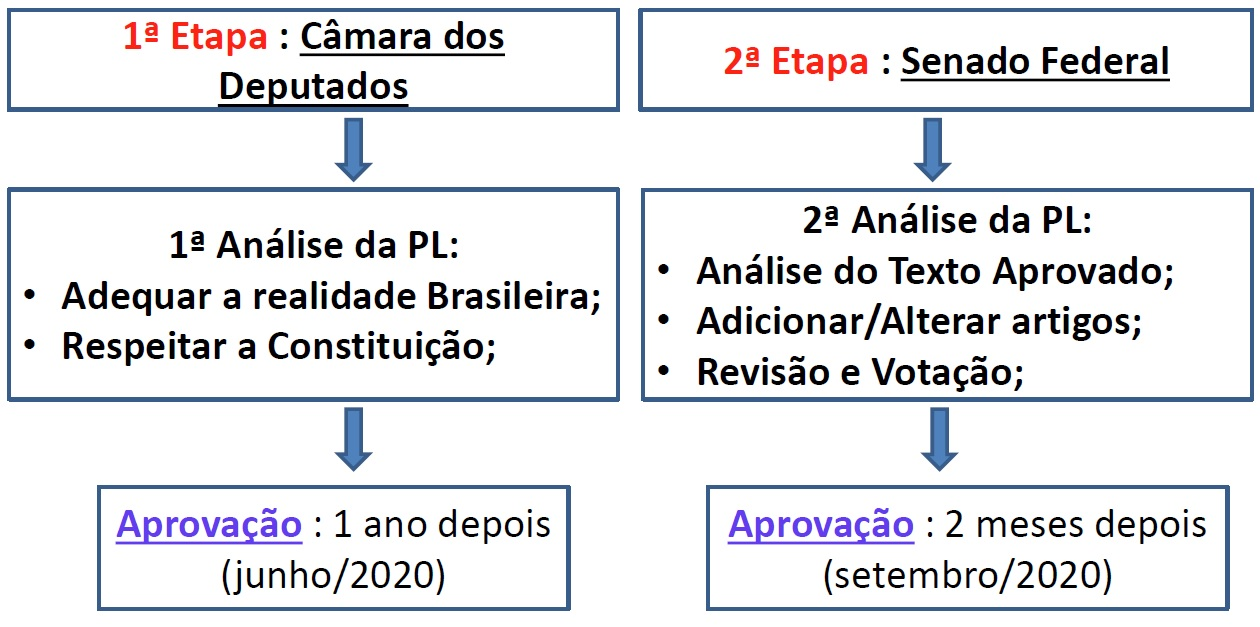
\includegraphics[height=.7\textheight]{etapa1.jpg}\\
            \vspace{-0.2cm}
            \caption{Primeira e Segunda Etapa que Antecederam a Aprovação da Lei n 14.071}\label{esquematabela1}}
        \end{figure}
\newpage
\begin{figure}[!htb]
            \centering{
            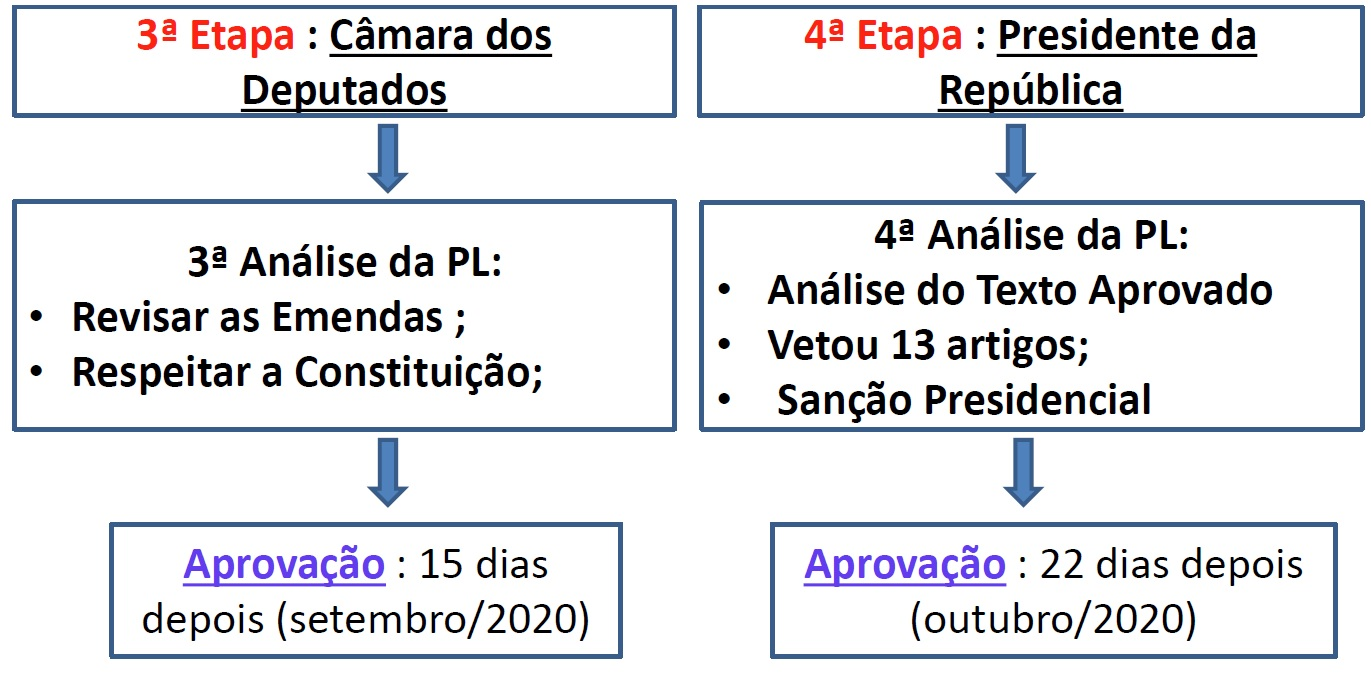
\includegraphics[height=.7\textheight]{etapa2.jpg}\\
            \vspace{-0.2cm}
            \caption{Terceira e Quarta Etapa que Antecederam a Aprovação da Lei n 14.071}\label{esquematabela1}}
        \end{figure}
\newpage
\begin{figure}[!htb]
            \centering{
            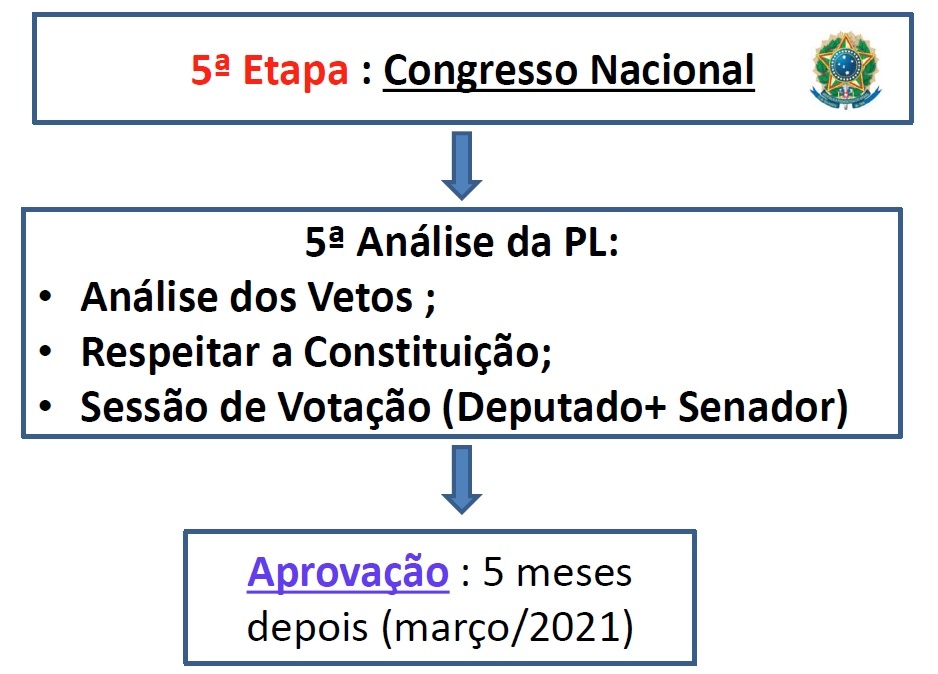
\includegraphics[height=.7\textheight]{etapa3.jpg}\\
            \vspace{-0.2cm}
            \caption{Quinta Etapa que Antecederam a Aprovação da Lei n 14.071}\label{esquematabela1}}
        \end{figure}   
%--------------------------------------------------------------------------------------------------------------------
\begin{frame}{Modificações na Lei}
    \begin{itemize}
        \item \justifying É a 39 lei a alterar o CTB, promovido pelo Projeto de Lei n 3.267/2019 transformado em Lei Ordinária n 14.071 e publicado em 14 de outubro de 2020;
        \item Foi a maior a publicação que trouxe 57 modificações;
        \item \justifying Modificações com 46 Alterações: 10, 12, 13, 19, 20, 21, 22, 24, 25, 29, 40, 64, 98, 101, 105, 106, 121, 131, 134, 138, 145, 147, 148-A, 158, 159, 161, 182, 208, 218, 220, 233, 244, 250, 257, 259, 261, 267, 268, 269, 270, 271, 282, 284, 285, 289 e Anexo I;
        \item  1(Um) artigo revogado por completo: 151;
        \item  \justifying 10(Dez) artigos incluídos: 10-A, 25-A, 44-A, 129-B, 134-A, 165-B, 268-A, 281-A, 282-A e 312-B;
        \item 6 artigos vetados: 56-A, 101, 147, 233-A, 244 e 268;
    \end{itemize}
\end{frame}
%----------------------------------------------------------------------------------------------------------------------

%----------------------------------------------------------------------------------------------------------------------
\section{Lei n 14.229/2021}
\subsection{41 Mudança no CTB}
\begin{frame}{Conceitos}
    \begin{itemize}
        \item \justifying Você conhece a Lei n 14.229/2021 – mais conhecida como Lei do Guincho;
        \item \justifying Trata-se de uma lei proposta pelo Ministério da Infraestrutura e Economia, em 2021, que visava a pequenas mudanças no CTB;
        \item \justifying Apresentado pela Secretaria Especial de Modernização do Estado(SEDEME) em maio de 2021, a Nova Lei iniciou seu caminho como Medida Provisória n 1.050/2021;
        \item \justifying Por fim, foram aprovadas medidas para o CTB que gerarão grandes impactos na vida do motorista brasileiro;
    \end{itemize}
\end{frame}
\begin{frame}{Modificações na Lei}
    \begin{itemize}
        \item \justifying É a 41 lei a alterar o CTB, promovido pelo Medida Provisória n 1.050/2021 transformado em Lei Ordinária n 14.299 e publicado em 21 de outubro de 2021;
        \item Foi a Publicação que trouxe 23 modificações;
        \item \justifying 14 Alterações: 2, 3, 20, 99, 101, 131, 257, 271, 282, 285, 289, 290, 338, Anexo1;
        \item 01 Artigo revogado p/completo: inciso 3 do art. 285;
        \item \justifying 08 Artigos Incluídos: 6-A, 9-A, 9-B, 9-C, 9-D, 289-A, 290A, e 338-A.;
    \end{itemize}
\end{frame}
\begin{frame}{Objetivos}{Promover Alterações e alinhamento nas seguintes Leis:}
    \begin{itemize}
        \item Lei n 9.503/1997;
        \item Lei n 7.408/1985;
        \item Lei n 10.029/2011;
        \item Constituição Federal de 1988;
    \end{itemize}
\end{frame}
%-------------------------------------------------------------------------------------------------------------------


%-------------------------------------------------------------------------------------------------------------------
\section{Lei n 14.304/2022}
\subsection{42 Mundança no CTB}
\begin{frame}{Introdução}
    \begin{itemize}
        \item \justifying A Lei n 14.304, veda a divulgação, a publicação ou a disseminação, em redes sociais ou em quaisquer outros meios de divulgação digitais, eletrônicos ou impressos, do registro visual da prática de infração que coloque em risco a segurança no trânsito;
        \item \justifying Altera a Lei n 9.503, de 23 de setembro de 1997 (Código de Trânsito Brasileiro);
        \item  Vetos: 1, 2, 3, 77-F, 261, 263, 280, 282, 298; 
        \item  Alteração: 281;
        \item  \justifying O novo regramento estabelece multa de R\$ 2.974,70 para quem descumprir a regra, além da Suspensão da Carteira Nacional de Habilitação por 12 meses;
    \end{itemize}
\end{frame}

\begin{frame}{Modificações}
    \begin{itemize}
        \item \justifying É a 42 lei a alterar o CTB, proveniente do Projeto de Lei n 130, de 2020 , de acordo com a Mensagem n 65, de 2022;
        \item Foi a publicação que trouxe vetos e alteração;
    \end{itemize}
\end{frame}
%------------------------------------------------------------------------------------------------------------------------


%------------------------------------------------------------------------------------------------------------------------
\section{Mudanças no CTB}
\subsection{Artigo 7}
\begin{frame}{Secretaria Nacional de Trânsito - SENATRAN}
    \begin{itemize}
        \item Órgão Máximo \textbf{\underline{EXECUTIVO}} de Trânsito;
        \item \justifying Órgão \textbf{\underline{SUBORDINADO}} a Secretaria Nacional de Transporte Terrestres do Ministério da Infraestrutura(Decretonº10.638/2020);
        \item \justifying O \textcolor{red}{\underline{DENATRAN}} passou a se chamar \textcolor{red}{\underline{SENATRAN}} (Decreto n 10.788/2021);
    \end{itemize}
\end{frame}

\begin{frame}{Competências 1 do SENATRAN}
    \begin{itemize}
        \item \justifying \textcolor{red}{Estabelecer Procedimentos} sobre a aprendizagem e habilitação de condutores de veículos, a expedição de documentos de condutores,de registro e licenciamento de veículos;
        \item \justifying \textcolor{red}{Expedir} a Permissão para dirigir, a CNH, os CRV e CRLV mediante delegação aos órgãos executivos dos Estados e do DF;
        \item \justifying \textcolor{red}{Expedir} a permissão internacional para conduzir veículos e o certificado de passagem nas alfandegas, mediante delegação aos órgãos executivos dos Estado e do DF ou a entidade habilitada para este fim pelo poder público federal.
    \end{itemize}
\end{frame}
\begin{frame}{Competências 2 do SENATRAN}
    \begin{itemize}
        \item \justifying \textcolor{red}{Organizar e Manter} o Registro de Carteira de Habilitação(RENACH);
        \item \justifying \textcolor{red}{Organizar e Manter} o Registro Nacional de Veículos Automotores(RENAVAN);
        \item \justifying \textcolor{red}{Organizar e Manter} o Registro Nacional de Infrações de Trânsito(RENAINF);
    \end{itemize}
\end{frame}
\begin{frame}{Policia Rodoviária Federal - PRF}
Competências 1:
    \begin{itemize}
        \item \justifying Realizar o patrulhamento ostensivo, executando operações relacionadas com segurança pública, como objetivo de preservar aordem, a incolumidade das pessoas, o patrimônio da União e o de terceiros.
        \item \justifying Executar a fiscalização de trânsito, aplicar as \textcolor{red}{Penalidades DE ADVERTÊNCIA POR ESCRITO e multa} e as medidas administrativas cabíveis, \textcolor{red}{com a notificação dos infratores e a arrecadação das multas aplicadas} e dos valores provenientes de estadia e remoção de veículos, objetos e animais e de escolta de veículos de cargas superdimensionadas ou perigosas;
    \end{itemize}
\end{frame}
\begin{frame}{Policia Rodoviária Federal - PRF}
Competências 2:
    \begin{itemize}
        \item \justifying \textcolor{red}{Efetuar} \textcolor{blue}{Levantamento} dos locais de acidentes de trânsito e dos serviços de atendimento, socorro e salvamento de vítimas;
        \item \justifying \textcolor{red}{Coletar} \textcolor{blue}{Dados Estatísticos} e elaborar estudos sobre acidentes de trânsito e suas causas, adotando ou indicando medidas operacionais preventivas e encaminhando-os ao órgão rodoviário federal.
        \item \justifying \textcolor{red}{Credenciar} \textcolor{blue}{os serviços de escolta}, \textcolor{red}{fiscalizar} e adotar \textcolor{blue}{medidas de segurança} relativas aos serviços de remoção de veículos, escolta e transporte de cargas indivisíveis.
    \end{itemize}
\end{frame}
\begin{frame}{Policia Rodoviária Federal - PRF}
Competências 3:
    \begin{itemize}
        \item \justifying \textcolor{red}{Implementar} as medidas da Política Nacional de Segurança e Educação de Trânsito;
        \item \justifying \textcolor{red}{Promover} e \textcolor{red}{Participar} de projetos e programas de educação e segurança, de acordo com as diretrizes estabelecidas pelo CONTRAN;
        \item \justifying \textcolor{red}{Aplicar a Penalidade de SUSPENSÃO DO DIREITO DE DIRIGIR}, quando prevista de forma específica para a infração cometida, e comunicar a aplicação da penalidade ao órgão máximo executivo de trânsito da União;
    \end{itemize}
\end{frame}
\begin{frame}{Conselho Nacional de Trânsito - CONTRAN}
    \begin{itemize}
        \item Órgão Máximo \textbf{\underline{NORMATIVO}} e \textbf{\underline{CONSULTIVO}} de Trânsito;
        \item \justifying Órgão \textbf{\underline{COLEGIADO}} do Ministério da Infraestrutura (Decreto n 10.638/2020);
        \item Sede no Distrito Federal;
    \end{itemize}
\end{frame}

\begin{frame}{Objetivos do CONTRAN}
    \begin{itemize}
        \item \justifying \textcolor{red}{Coordenar} os Órgãos do Sistema Nacional de Trânsito, objetivando a integração de suas atividades; 
        \item \justifying \textcolor{red}{Estabelecer} as normas regulamentares referidas neste Código e as diretrizes da Politica Nacional de Trânsito.
    \end{itemize}
\end{frame}


\subsection{Artigo 10}
\begin{frame}{Composição do CONTRAN (Art.10)}
È composto pelos Ministros de Estado:
    \begin{itemize}
        \item Da Infraestrutura (Que é o Presidente);
        \item Da Ciência, Tecnologia e Inovações;
        \item Da Educação;
        \item Da Defesa;
        \item Do Meio-Ambiente; 
        \item Das Relações Exteriores;
        \item Da Economia
        \item Da Saúde;
        \item Da Justiça e Segurança Pública;
        \item Da Agricultura, Pecuária e Abastecimento; 
    \end{itemize}
\end{frame}
\begin{frame}{Artigo 10 Inciso 4}
    \begin{itemize}
        \item \justifying Os Ministros de Estado deverão indicar suplente, que será servidor de nível hierárquico igual ou superior ao nível 6 do Grupo-Direção e Assessoramento Superiores-DAS ou, no caso do Ministério da DEFESA, alternativamente, OFICIAL-GERAL.
    \end{itemize}
\end{frame}
\begin{frame}{Artigo 10 Inciso 5}
    \begin{itemize}
        \item \justifying Compete ao DIRIGENTE do órgão máximo executivo de trânsito da União (\textcolor{red}{\underline{DENATRAN}}) atuar como Secretário Executivo do CONTRAN.
    \end{itemize}
\end{frame}
\begin{frame}{Artigo 10 Inciso 6}
    \begin{itemize}
        \item \justifying O quórum de \textbf{\underline{Votação}} e de \textbf{\underline{Aprovação}} no CONTRAN é o de \textcolor{red}{MAIORIA ABSOLUTA (metade+1)}.
    \end{itemize}
\end{frame}
\begin{frame}{Artigo 10-A}
    \begin{itemize}
        \item \justifying \textbf{\underline{PODERÃO}} ser convidados aparticipar der euniões do CONTRAN, \textcolor{red}{Sem Direito a Voto}, representantes de órgãos e entidades setoriais responsáveis ou impactados pelas propostas ou matérias em exame.
    \end{itemize}
\end{frame}
\subsection{Artigo 12}
\begin{frame}{Consulta Pública (Art.12)}
Compete ao CONTRAN:
    \begin{itemize}
        \item \justifying  I- estabelecer a normas regulamentares referidas neste código e as diretrizes da Política Nacional de Trânsito;
    \end{itemize}
\end{frame}
\begin{frame}{Artigo 12 Inciso I}
    \begin{itemize}
        \item \justifying As propostas de normas regulamentares de que se trata o inciso I do caput deste artigo serão submetidas a \textbf{\underline{Prévia Consulta Pública}}, por meio de rede mundial de computadores, pelo período \textcolor{red}{mínimo de 30(trinta) dias}, antes do exame da matéria pelo Contran.
    \end{itemize}
\end{frame}
\begin{frame}{Artigo 12 Inciso II}
    \begin{itemize}
        \item \justifying As contribuições recebidas na consulta pública de que tratao §1º deste artigo ficarão à disposição pelo prazode 02(dois) anos, contado da data de encerramento da consulta pública.
    \end{itemize}
\end{frame}
\begin{frame}{Artigo 12 Inciso III}
    \begin{itemize}
        \item \justifying Em caso de urgência e de relevante interesse público, o presidente do CONTRAN poderá editar de liberação, ad referendum do Conselho e comprazo de validade máximade 90(noventa) dias, para estabelecer norma regulamentar prevista no inciso I do caput, dispensado o cumprimento do dispositivo nos §§1º e 2º deste artigo, vedada a reedição.
    \end{itemize}
\end{frame}
\begin{frame}{Artigo 12 Inciso IV}
    \begin{itemize}
        \item \justifying Encerrado o prazo previsto no inciso terceiro deste artigo sem o refendo do Contran, adeliberação perderá a sua eficácia e permanecerão válido os efeitos dela decorrentes.
    \end{itemize}
\end{frame}
\begin{frame}{Artigo 12 Inciso V}
    \begin{itemize}
        \item \justifying Norma do Contran poderá dispor sobre o uso de sinalização horizontal ou vertical que utilize técnicas de estímulos comportamentais para a redução de acidentes de trânsito;
    \end{itemize}
\end{frame}
\subsection{Artigo 13}
\begin{frame}{Câmaras Técnicas (Art.13)}
Compete as Camâras Técnicas:
    \begin{itemize}
        \item \justifying As Câmaras Temáticas, órgãos técnicos vinculados ao CONTRAN, são integradas por especialistas e têm como objetivo estudar e oferecer sugestões e embasamento técnico sobre assuntos específicos para decisões daquele colegiado.
    \end{itemize}
\end{frame}
\begin{frame}{Artigo 13 Inciso I}
    \begin{itemize}
        \item \justifying Cada câmara é constituída por ESPECIALISTAS representes de órgãos e entidades executivos da União, dos Estados, ou do Distrito Federal e dos Municípios, EM IGUAL NÚMERO, pertencentes ao Sistema Nacional de Trânsito, além de especialistas representantes dos diversos segmentos da sociedad e relacionados como trânsito, todos indicados segundo regimento específico definido pelo CONTRAN e designados pelo ministro ou dirigente coordenador máximo do SNT.
    \end{itemize}
\end{frame}
\begin{frame}{Artigo 13 Inciso II}
    \begin{itemize}
        \item \justifying Os segmentos da sociedade, relacionados no parágrafo anterior, serão representados por PESSOA JURÍDICA e devem atender aos requisitos estabelecidos pelo CONTRAN.
    \end{itemize}
\end{frame}
\begin{frame}{Artigo 13 Inciso III}
    \begin{itemize}
        \item \justifying A coordenação das Câmaras Temáticas será exercida por representantes do órgão máximo executivo de trânsito da União ou dos Ministérios representados pelo Contran, conforme definido no ato de criação de cada Câmara Temática;
    \end{itemize}
\end{frame}
\subsection{Artigo 22}
\begin{frame}{Parágrafo Ùnico - Inciso III}
\justifying 
As competências no inciso II do caput deste artigo relativas ao processo de suspensão de condutores serão exercidas quando:
    \begin{itemize}
        \item \justifying Vistoriar, inspecionar quanto as condições de segurança veicular, registrar, emplacar, selar a placa, e licenciar veículos, expedindo o CRV e CRLV, mediante delegação do órgão federal competente;
    \end{itemize}
\end{frame}
\subsection{Artigo 24}
\begin{frame}{Artigo 24 - Inciso VI}
Òrgãos Executivo Municipal
    \begin{itemize}
        \item \justifying Executar a \textcolor{red}{\textbf{fiscalização}} de trânsito em vias terrestres, edificações de uso publico e edificações privadas de uso coletivo,  \textcolor{red}{\textbf{Autuar}} e  \textcolor{red}{\textbf{aplicar as medidas administrativas cabíveis e as penalidades de advertência por escrito e multa}}, por infrações de circulação, estacionamento e parada prevista neste Código, no exercício regular do poder de policia de trânsito, notificando os infratores e arrecadando as multas que aplicar,exercendo iguais atribuições no âmbito de edificações privadas de uso coletivo, somente para infrações de uso de vagas reservadas em estacionamentos;
    \end{itemize}
\end{frame}
\begin{frame}{Artigo 24 - Inciso VIII}
    \begin{itemize}
        \item \justifying Fiscalizar, autuar e aplicar as penalidades e medidas administrativas cabíveis relativas a infrações por excesso de peso, dimensões e lotação dos veículos, bem, como notificar e arrecadar as multas que aplicar;
    \end{itemize}
\end{frame}
\begin{frame}{Artigo 24 - Inciso XXII}
    \begin{itemize}
        \item \justifying \textcolor{red}{\textbf{Aplicar a penalidade de suspensão do direito de dirigir}}, quando prevista de forma específica para a infração cometida, e comunicar a aplicação da penalidade ao órgão máximo executivo de trânsito da união.
    \end{itemize}
\end{frame}

\begin{frame}{Artigo 24 - Inciso XXIII}
    \begin{itemize}
        \item \justifying Criar, implantar e manter \textcolor{red}{\textbf{ESCOLAS PÚBLICAS DE TRÂNSITO}}, destinados a educação de crianças e adolescentes, por meio de aulas teóricas e práticas sobre legislação, sinalização e comportamento no trânsito.
    \end{itemize}
\end{frame}
\subsection{Artigo 25A}
\begin{frame}{Polícia do Lesgislativo Federal}
    \begin{itemize}
        \item \justifying Os agentes dos órgãos policiais da Câmara dos Deputados e do Senado Federal, a que se referem o inciso IV do caput do art.51 e o inciso XIII do caput do art.52 da Constituição Federal, respectivamente, mediante convenio como órgão ou entidade de trânsito com circunscrição sobre a via, poderão lavrar auto de infração de trânsito e remetê-lo ao órgão competente, nos casos em que a infração cometida nas adjacências do Congresso Nacional ou nos locais sob sua responsabilidade comprometer objetivamente os serviços ou colocarem risco a incolumidade das pessoas ou o patrimônio das respectivas Casas Legislativas.
    \end{itemize}
\end{frame}






%------------------------------------------------------------------------------------------------------------------------







\begin{frame}
    \begin{center}
        {\Huge\calligra Thank You}
    \end{center}
\end{frame}









\end{document}